\documentclass{article}
\usepackage[utf8]{inputenc}
\usepackage{datetime}
\usepackage{enumerate}
\usepackage{textcomp}
\usepackage{amsmath}
\usepackage{tikz}
\usetikzlibrary{arrows}
\usepackage{graphicx}
\graphicspath{ {./images/} }

\title{\bf \Large ASSIGNMENT 1}
\author{Xinhao Luo}
\date{\today}

\def\math#1{$#1$}

\setlength{\textheight}{8.5in}
\setlength{\textwidth}{6.5in}
\setlength{\oddsidemargin}{0in}
\setlength{\evensidemargin}{0in}
\voffset0.0in

\begin{document}
\maketitle
\medskip

\section{Exercise 1.3}
\begin{enumerate}[a)]
    \item Since \math{x(t)} is misclassified by \math{w(t)} at this time, the output \math{w^{T}x(t)} does not have the same sign as answer \math{y(t)}. The product between two numbers of different sign must be negative, thus less than 0 in this case.
    \item From (1.3), we have \math{w(t+1) = w(t) + y(t)x(t)}. Refer back to the original inequality: 
    \begin{equation}
        \begin{split}
            y(t)w^{T}(t + 1)x(t) &= y(t)w^{T}(t)x(t) + {x(t)y(t)}^{2}
        \end{split}
    \end{equation}
    Since \math{{x(t)y(t)}^{2}} will be a positive number, any number plus an positive number will be larger than itself. Thus, \math{y(t)w^{T}(t + 1)x(t) > y(t)w^{T}(t)x(t)}
    \item From section 1.3b, we know that \math{y(t)w^{T}(t + 1)x(t) > y(t)w^{T}(t)x(t)}. Here, \math{w^{T}(t)x(t)} is our predict result, and \math{y(t)} is the answer. Since the \math{y(t)w^{T}(t)x(t)} is becoming larger and larger each time, it is approaching positive each time \math{t} increase. Positive result means that output \math{w^{T}(t)x(t)} has the same sign as \math{y(t)}, the answer, which is the correct direction we would like to approach.
\end{enumerate}

\section{Exercise 1.5}
\begin{enumerate}[a)]
    \item Learning approach
    \item Design approach
    \item Learning approach
    \item Design approach
    \item Learning approach
\end{enumerate}

\section{Exercise 1.6}
\begin{enumerate}[a)]
    \item Supervised learning. Training data could be other users' profile with  their purchase history
    \item Reinforcement learning. Training data could be game steps with end result, and the result is not necessary always win/lose.
    \item Unsupervised learning. Training data could be a bunch of movies' metadata.
    \item Reinforcement learning. Training data could be music clips and their scores by public audience, the scores can be diverse.
    \item Supervised learning. Training data could be customers' credit profile, containing the amount of debts they have paid, or not paid.
\end{enumerate}

\section{Exercise 1.7}
\begin{enumerate}[a)]
    \item The picked function g will return black dot all the time, and its performance will be: \math{f_1} agrees with 0 points; \math{f_2, f_3, f_5} agree with 1 points; \math{f_4, f_6, f_7} agree with 2 points; \math{f_8} agrees with 3 points. 
    \item The picked function g will return white dot all the time, and its performance will be: \math{f_1} agrees with 3 points; \math{f_2, f_3, f_5} agree with 2 points; \math{f_4, f_6, f_7} agree with 1 points; \math{f_8} agrees with 0 points.
    \item XOR Performance: \math{f_7} agrees with 0 points; \math{f_3, f_5, f_8} agrees with 1 points ;\math{f_1, f_4, f_6} agree with 2 points; \math{f_2} agrees with 3 points
    \item The one disagree most with XOR will have the reverse function match with XOR, so its performance will be: 1 agree with 3 points, 3 agree with 2 points, 3 agrees with 1 point, and 1 agree with 0 point
\end{enumerate}

\section{Problem 1.1}

If we want to have the second ball in the bag also a black ball, it must be the bag with 2 black ball at the beginning. Here we set this bag as BB and the other one as BW.

\begin{equation}
    \begin{split}
        P(Bag BB \vert Picked Black Ball) &= \frac{P(Bag BB)P(Picked Black Ball \vert Bag BB)}{P(Picked Black Ball)} \\
        &= \frac{P(Picked Black Ball \& Bag BB)}{P(Picked Black Ball)} \\
        &= \frac{\frac{1}{2}}{\frac{2 + 1}{4}} \\
        &= \frac{2}{3}
    \end{split}
\end{equation}

\section{Problem 1.2}

\begin{enumerate}[a)]
    \item 
        \begin{itemize}
            \item Assuming our line \math{w_0 + w_1x_1 + w_2x_2 = 0} separating \math{h(x) = +1} and \math{h(x) = -1} exists. As we know that \math{h(x) = sign(w^Tx)}, the time where \math{h(x) = + 1}, \math{(w^Tx) > 0 }, then \math{(x_1, x_2)} will stay above the line, and vice versa, so it can be concluded that the line exists. 
            \item \begin{equation}
                \begin{split}
                    w_0 + w_1x_1 + w_2x_2 &= 0 \\
                    w_2x_2 &= -w_0 - w_1x_1 \\
                    x_2 &= -\frac{w_0}{w_2} - \frac{w_1}{w_2}x_1 \\
                    x_2 &= -\frac{w_1}{w_2}x_1 -\frac{w_0}{w_2}
                \end{split}
            \end{equation}
            So we have \math{a = -\frac{w_1}{w_2}} and \math{b = -\frac{w_0}{w_2}}
        \end{itemize}
    \item 
        \begin{enumerate}[1)]
            \item For \math{w = [1,2,3]^T}, we have \math{a = - \frac{2}{3}} and \math{b = - \frac{1}{3}} \\
            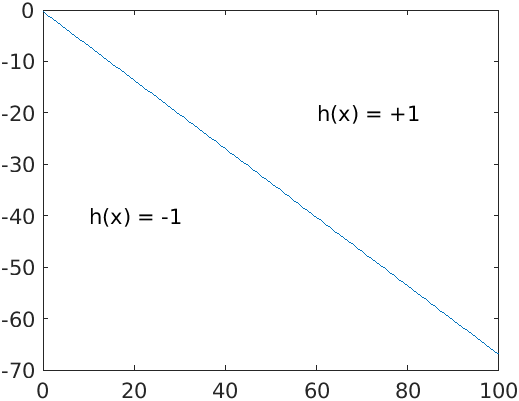
\includegraphics{1.2/1}
            \item For \math{w = - [1,2,3]^T}, we have the same line as above but different regions. \\
            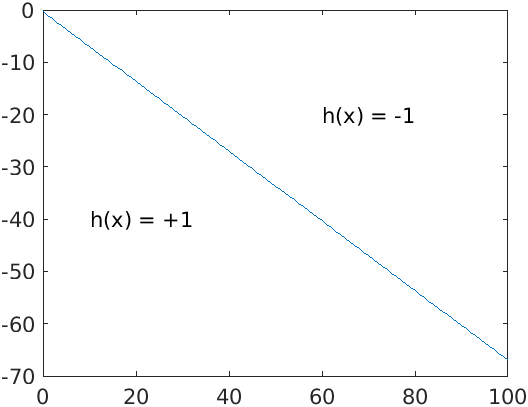
\includegraphics{1.2/2}
        \end{enumerate}
\end{enumerate}

\section{Problem 1.4}

\begin{enumerate}[a)]
    \item 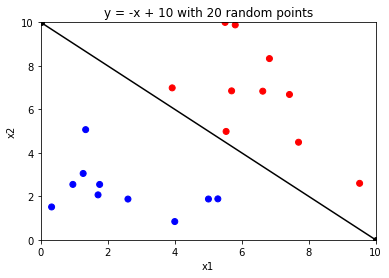
\includegraphics{1.4/1} \\ Note: red dots are \math{+1} and blue dots are -1
    \item 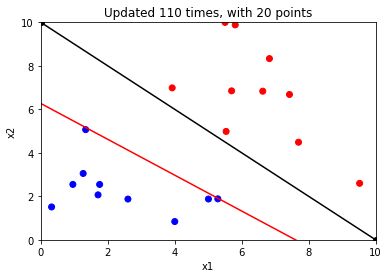
\includegraphics{1.4/2} \\ Comment: there is still an obvious gap between our target function and hypothesis.
    \item 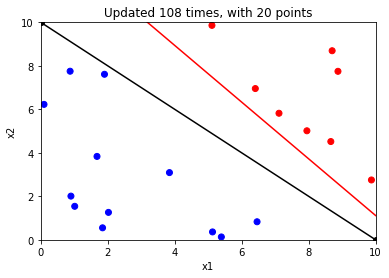
\includegraphics{1.4/3} \\ Compare: less times used but the gap is still obvious.
    \item 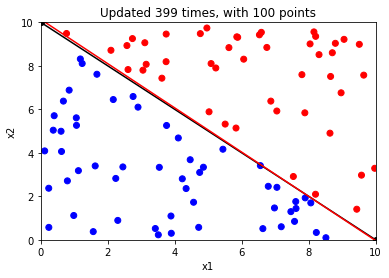
\includegraphics{1.4/4} \\ Compare: take more times to converge but the gap is far less obvious
    \item 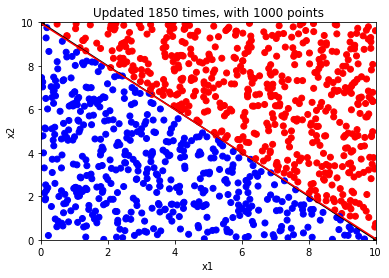
\includegraphics{1.4/5} \\ Compare: take a lot more times to converge but two functions are nearly identical.
\end{enumerate}

\end{document}
